The nuisance parameter pulls and constraints are compared among three fits (blinded background-only data fit, unblinded background-only data fit, and unblinded signal+background data fit) in Figures \ref{fig:comparison_NP_instrumental}, \ref{fig:comparison_NP_ttbar}, and \ref{fig:comparison_NP_other}.

\begin{figure}[htbp!]
  \centering
  \begin{subfigure}[t]{0.32\textwidth}
    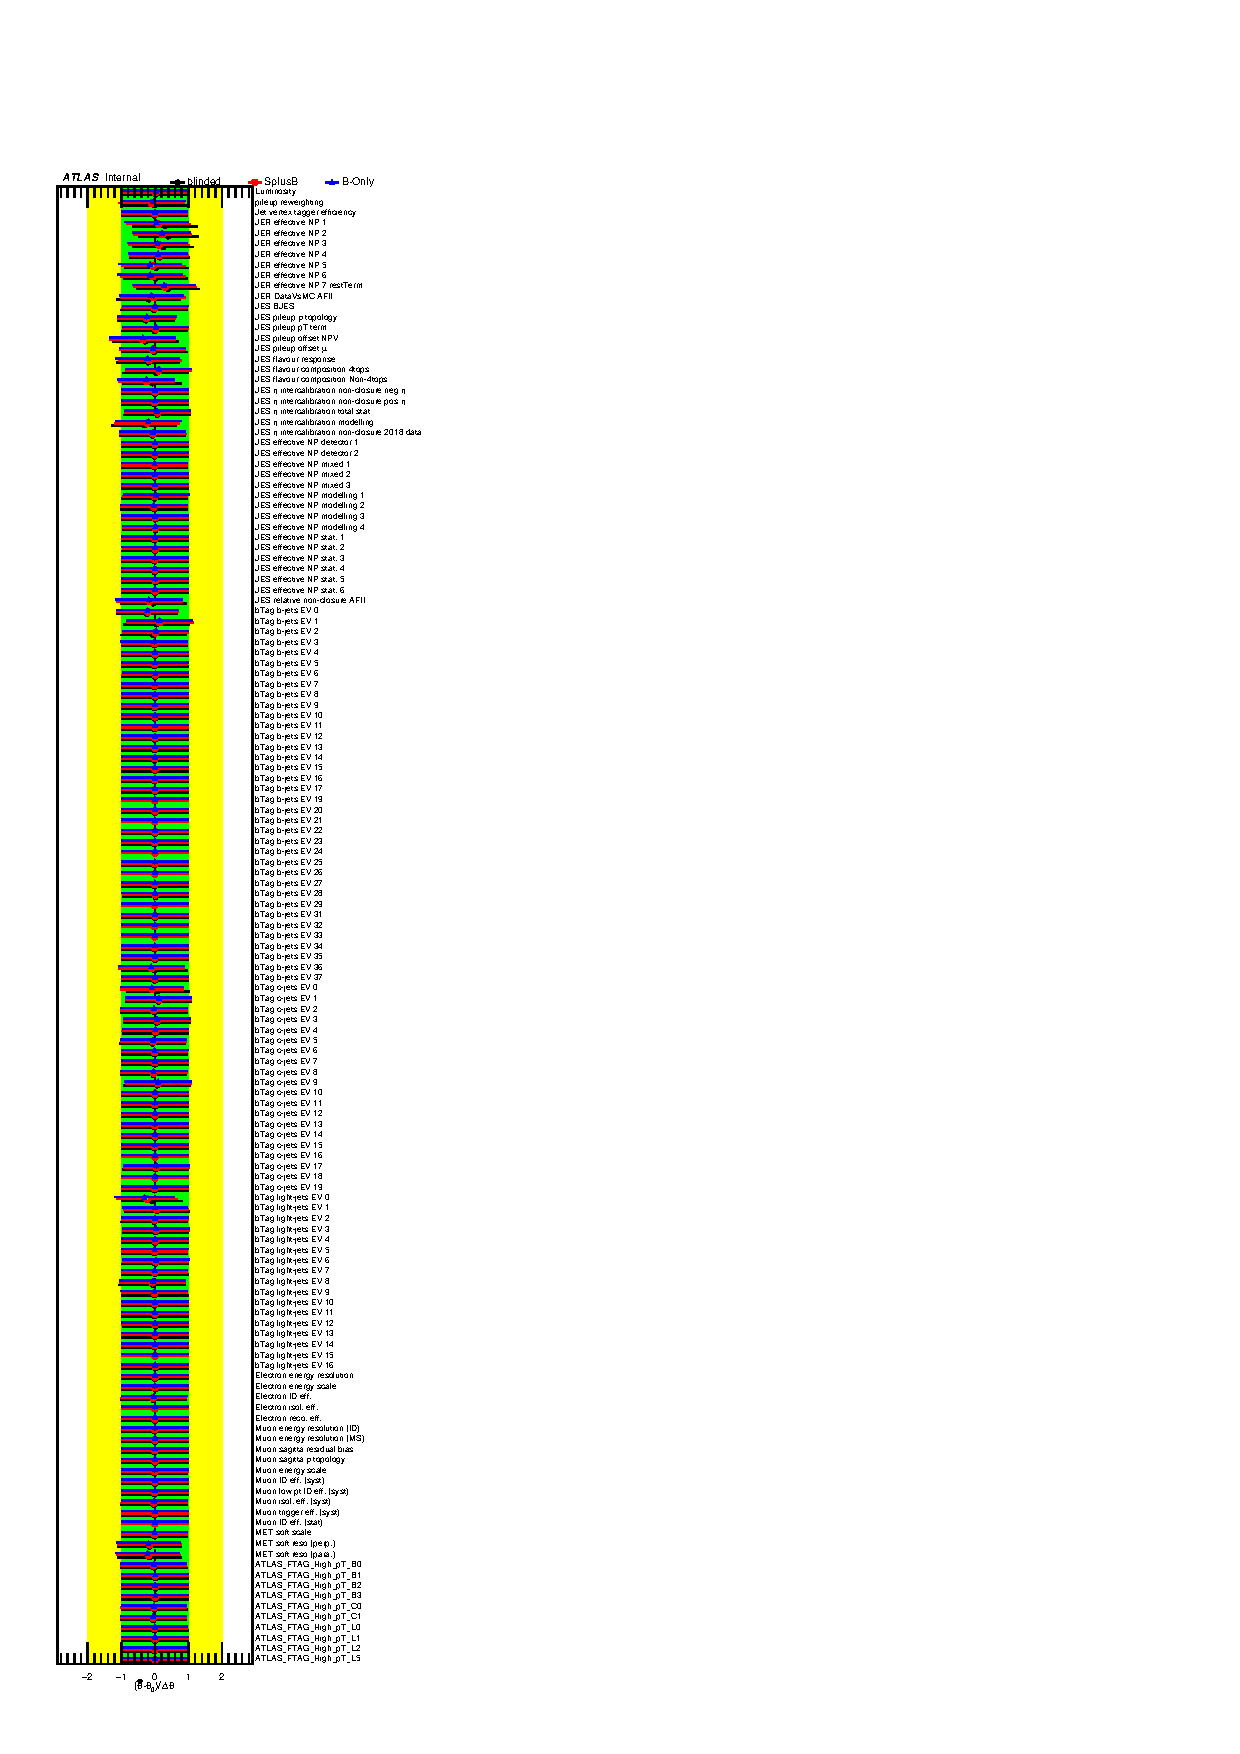
\includegraphics[width=\linewidth]{figures/fits/comparisons/fitTypes/400/all/comparison_data/NuisPar_comp_Instrumental.pdf}
    \subcaption{mH=400\gev}
  \end{subfigure}
  \begin{subfigure}[t]{0.32\textwidth}
    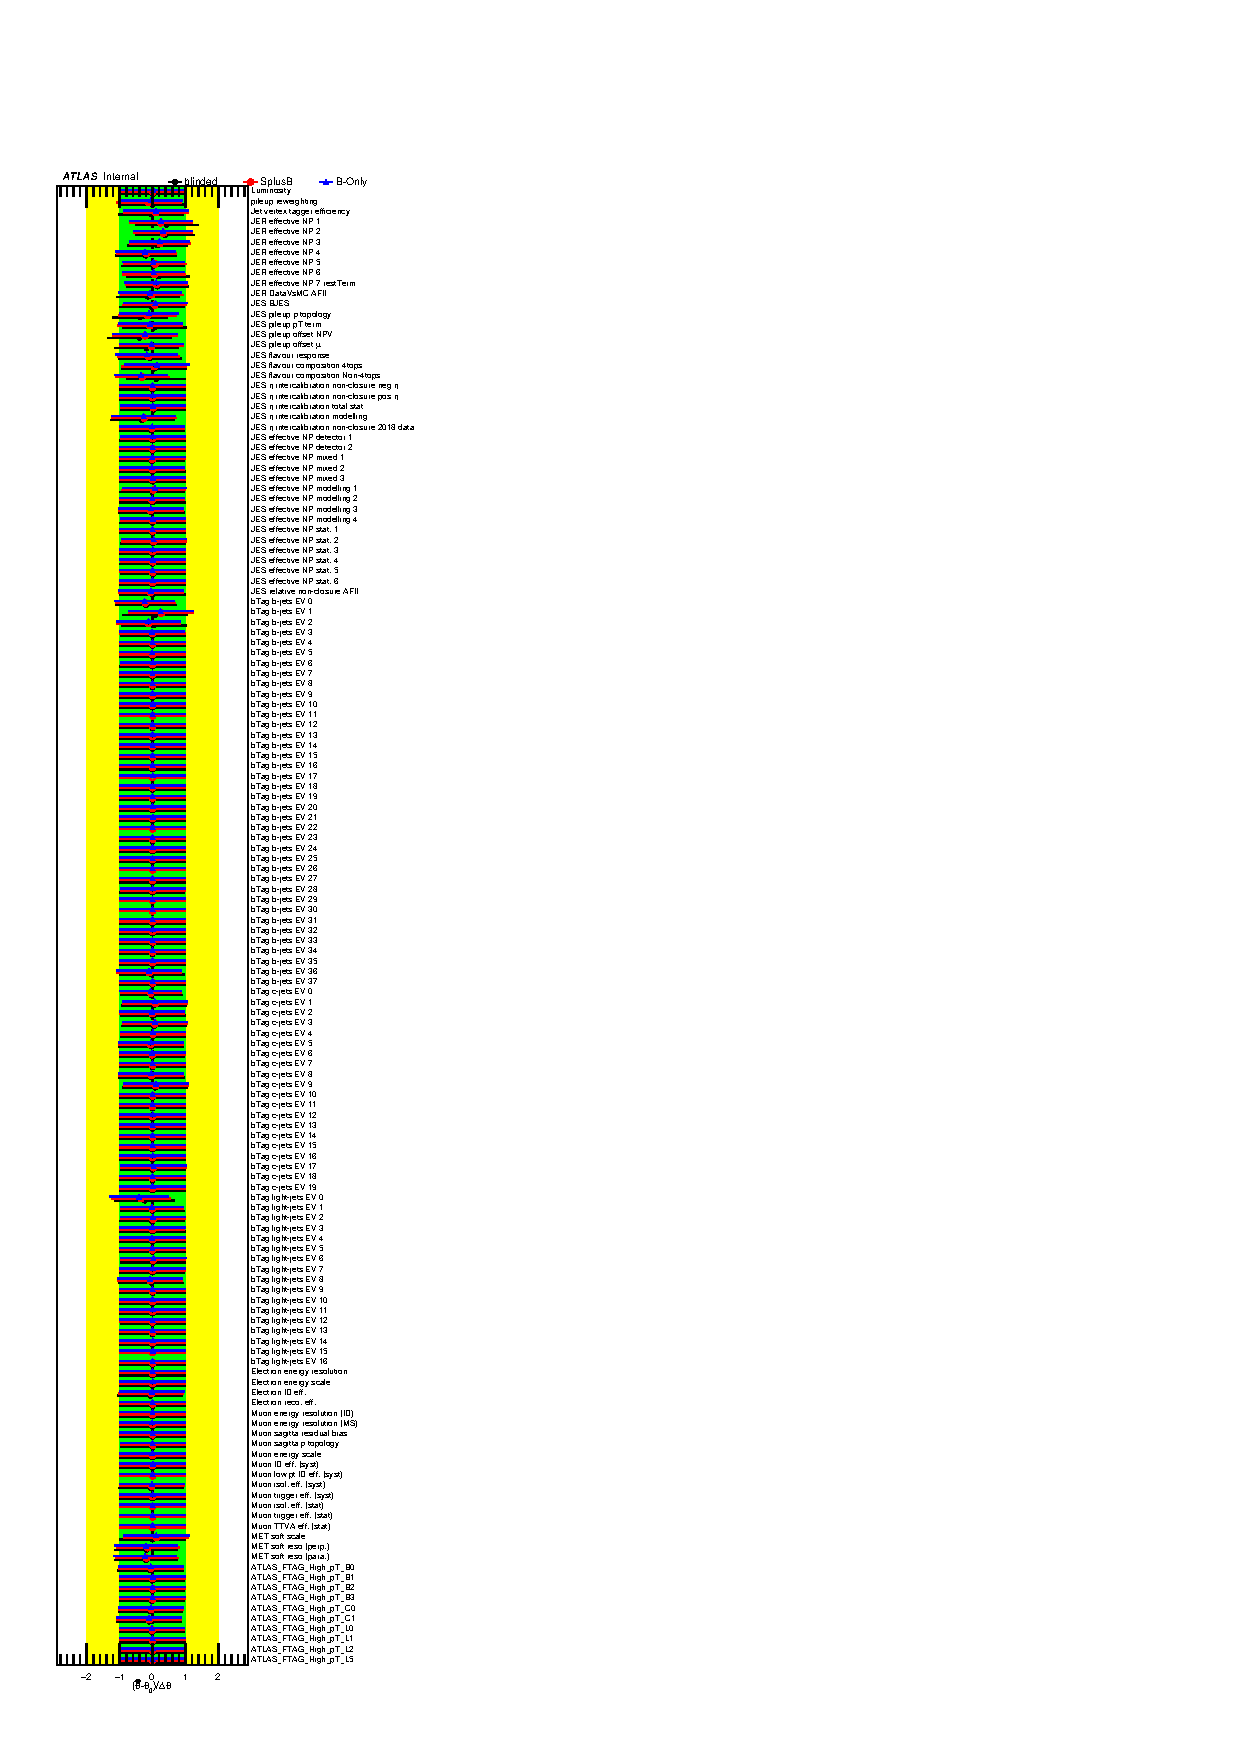
\includegraphics[width=\linewidth]{figures/fits/comparisons/fitTypes/700/all/comparison_data/NuisPar_comp_Instrumental.pdf}
    \subcaption{mH=700\gev}
  \end{subfigure}
  \begin{subfigure}[t]{0.32\textwidth}
    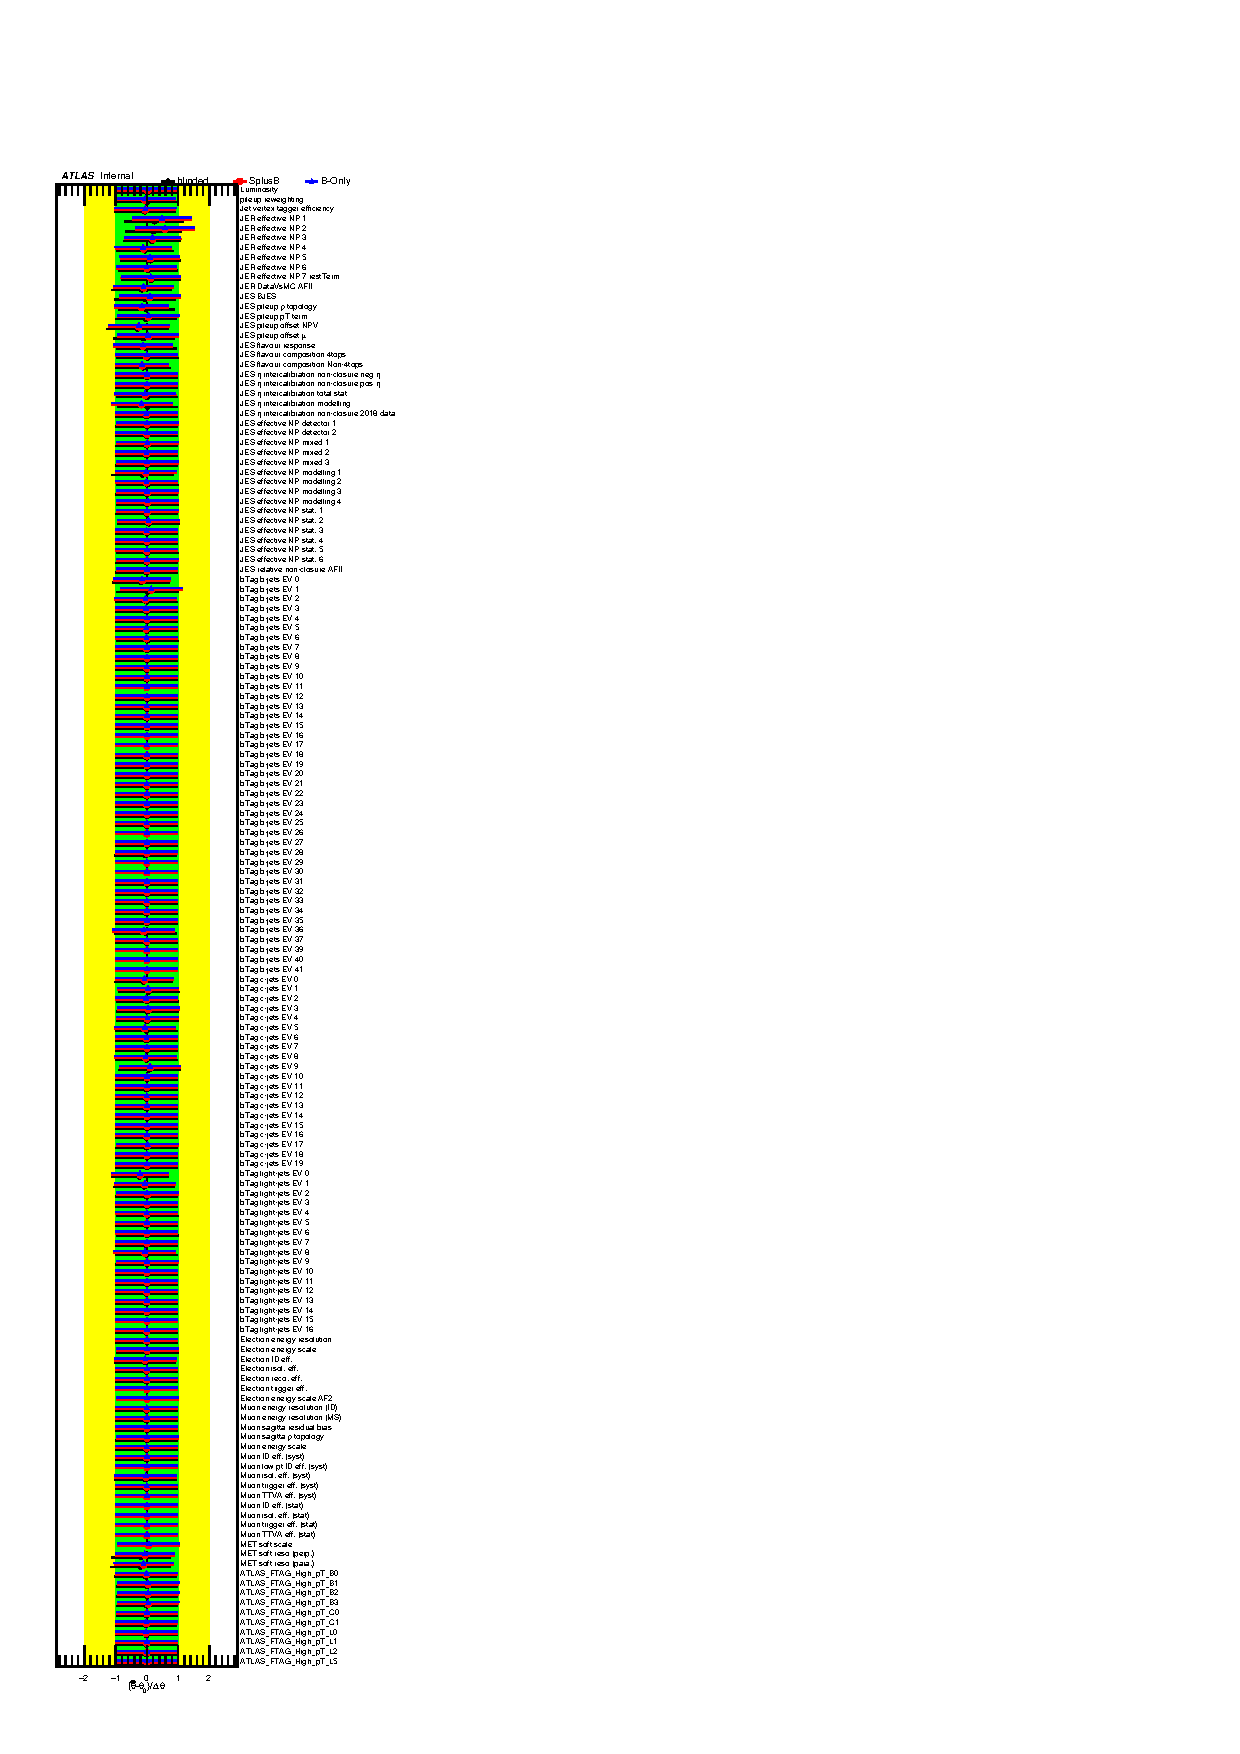
\includegraphics[width=\linewidth]{figures/fits/comparisons/fitTypes/1000/all/comparison_data/NuisPar_comp_Instrumental.pdf}
    \subcaption{mH=1000\gev}
  \end{subfigure}
  \caption{\label{fig:comparison_NP_instrumental}Fitted pulls and constraints for the nuisance parameters corresponding to the instrumental systematic uncertainties for combined Data fits for three mass points. Comparison is done for three fits: blinded background-only data fit, unblinded background-only data fit, and unblinded signal+background data fit.}
\end{figure}

\begin{figure}[htbp!]
  \centering
  \begin{subfigure}[t]{0.32\textwidth}
    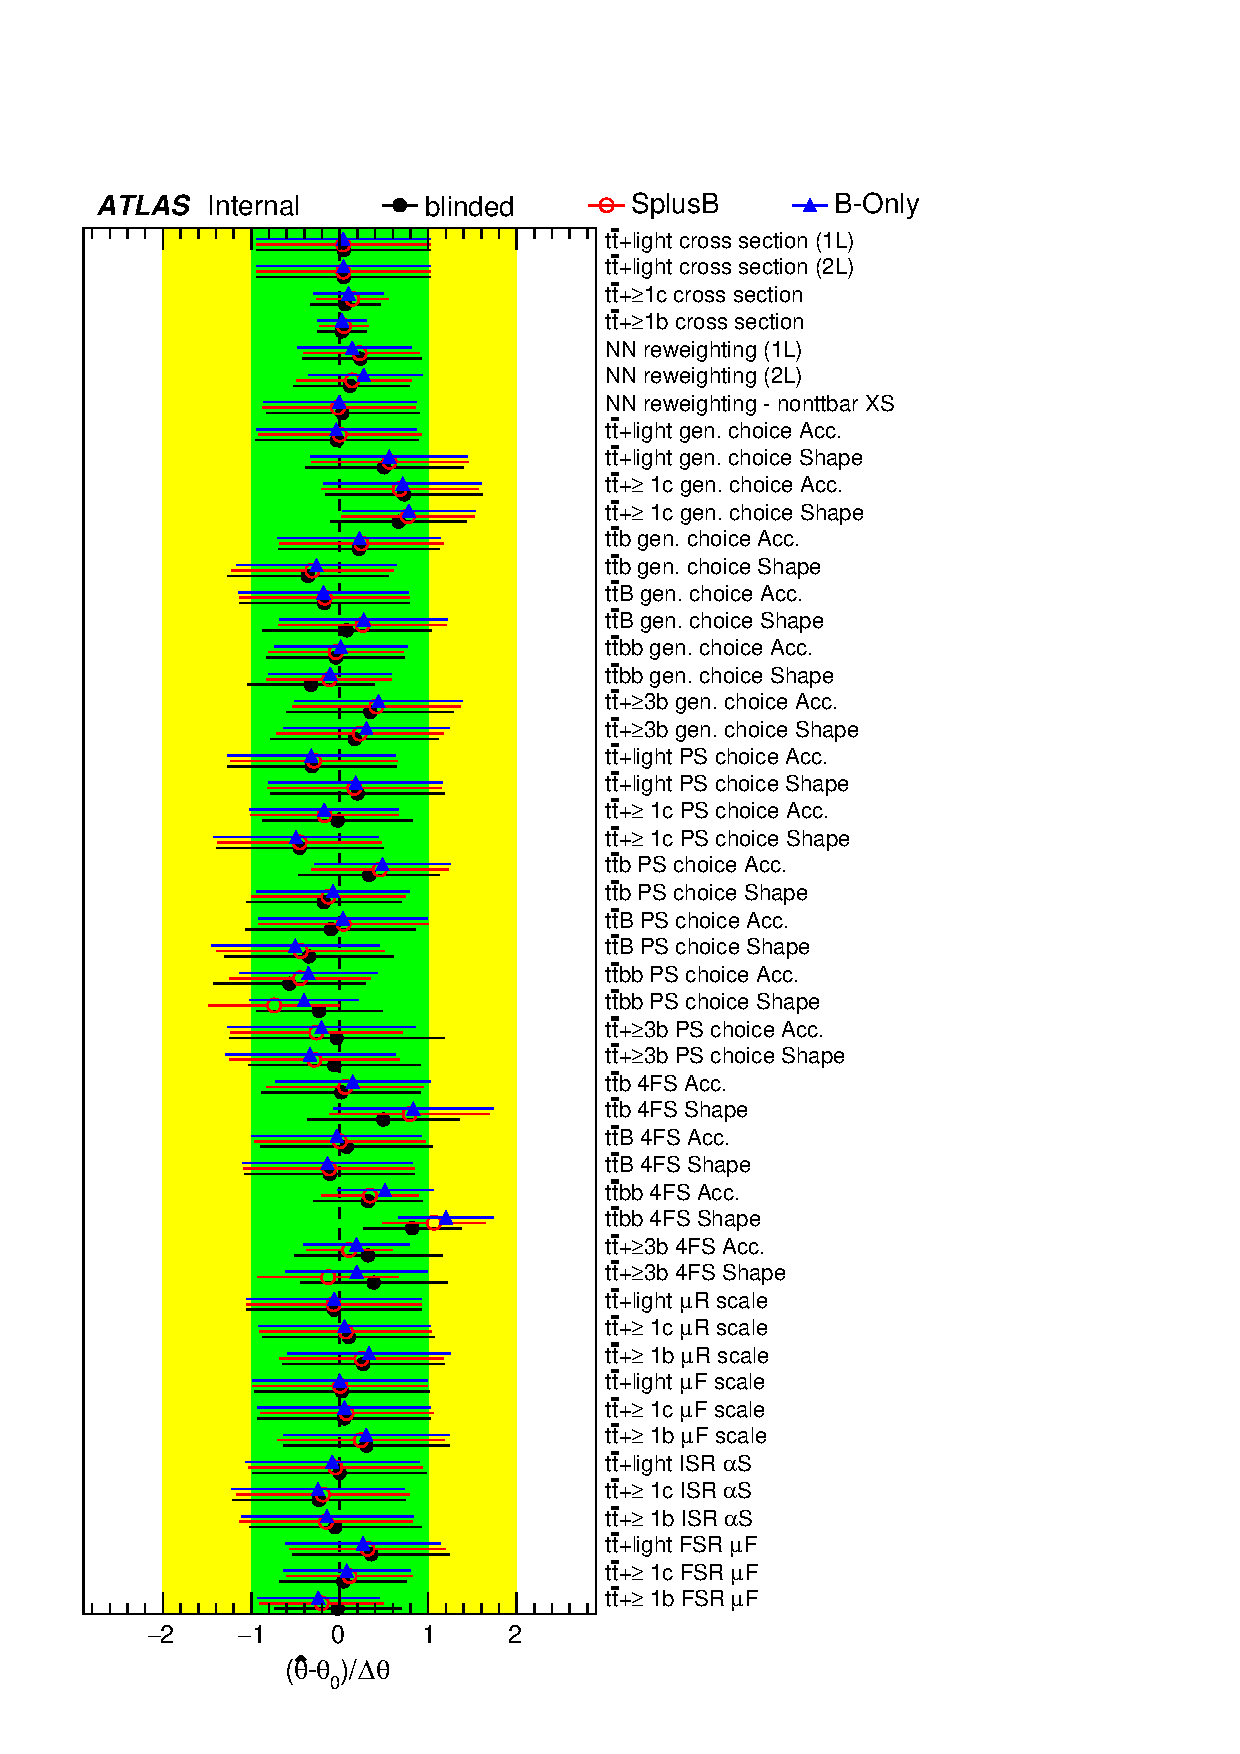
\includegraphics[width=\linewidth]{figures/fits/comparisons/fitTypes/400/all/comparison_data/NuisPar_comp_ttbar.pdf}
    \subcaption{mH=400\gev}
  \end{subfigure}
  \begin{subfigure}[t]{0.32\textwidth}
    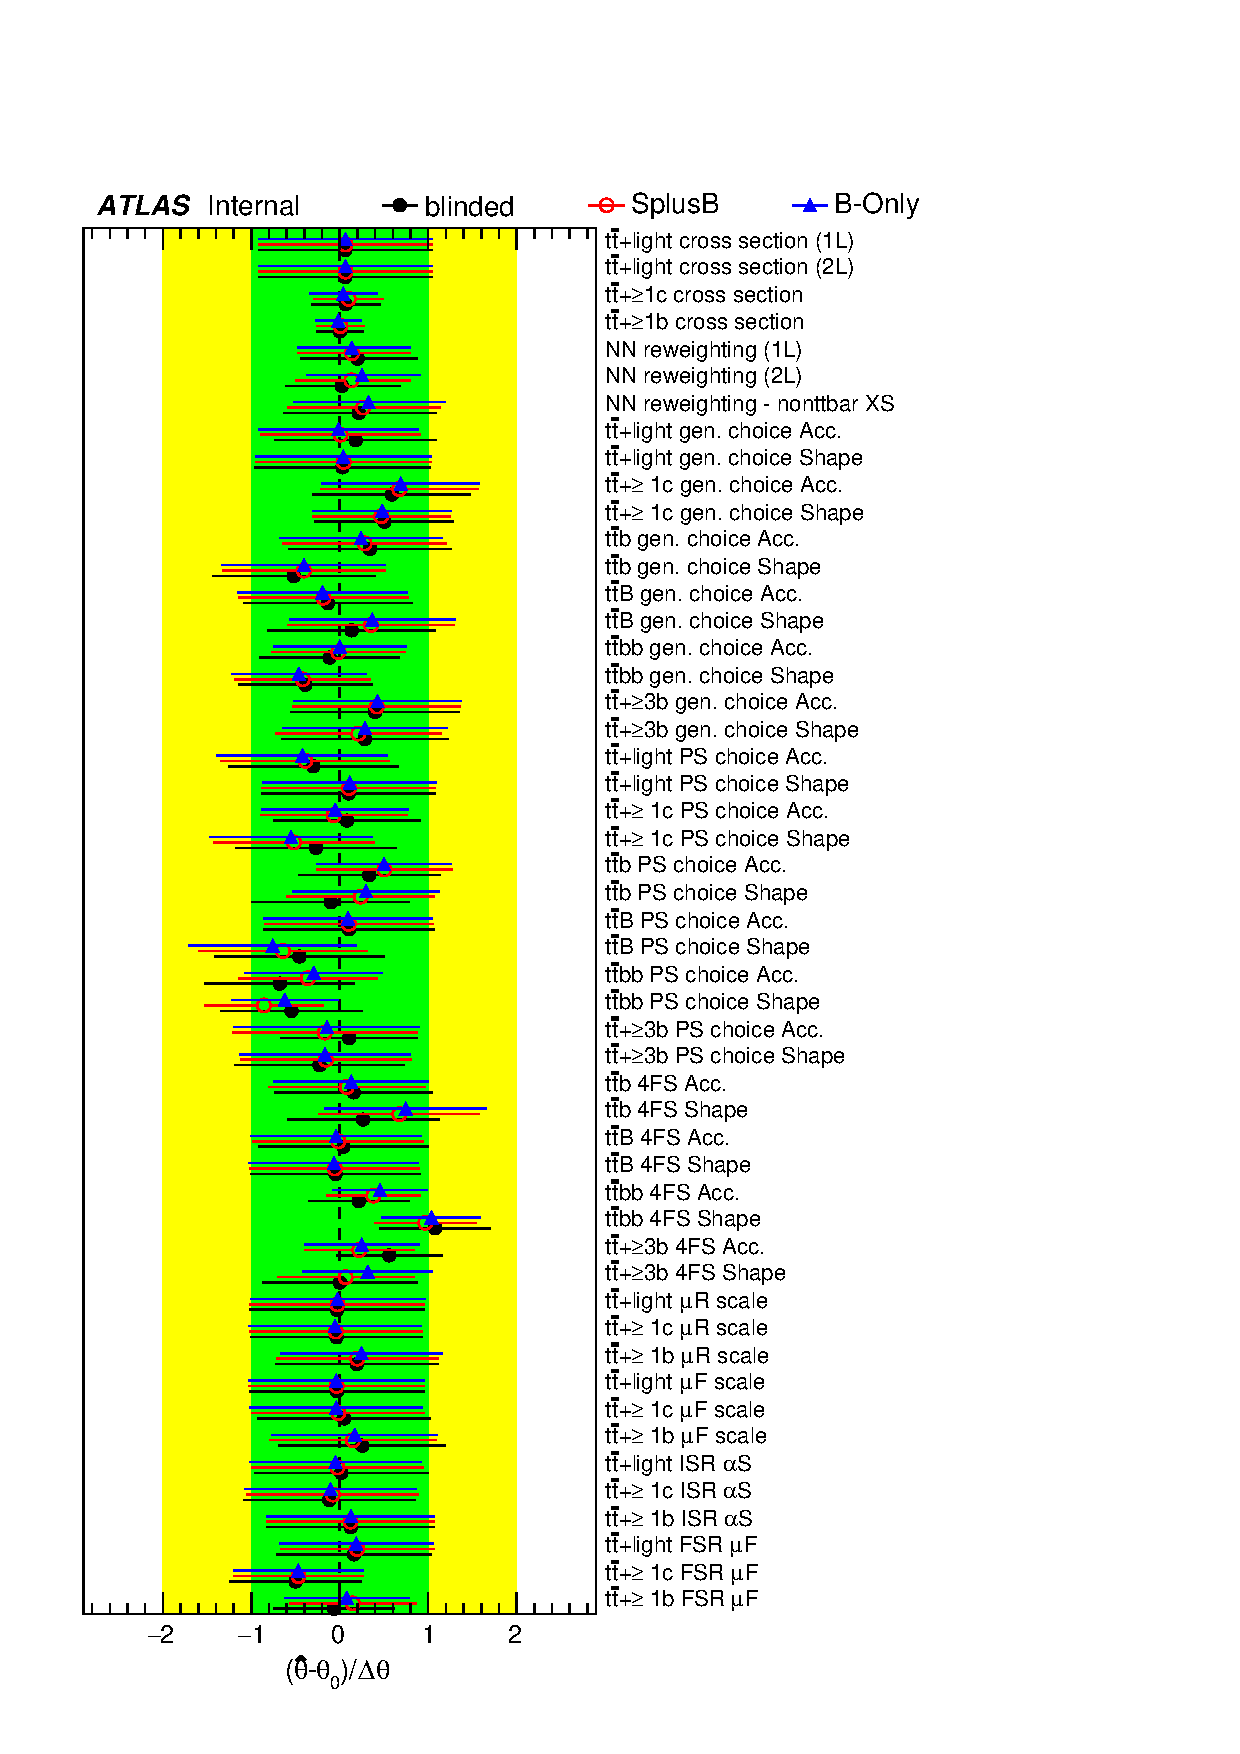
\includegraphics[width=\linewidth]{figures/fits/comparisons/fitTypes/700/all/comparison_data/NuisPar_comp_ttbar.pdf}
    \subcaption{mH=700\gev}
  \end{subfigure}
  \begin{subfigure}[t]{0.32\textwidth}
    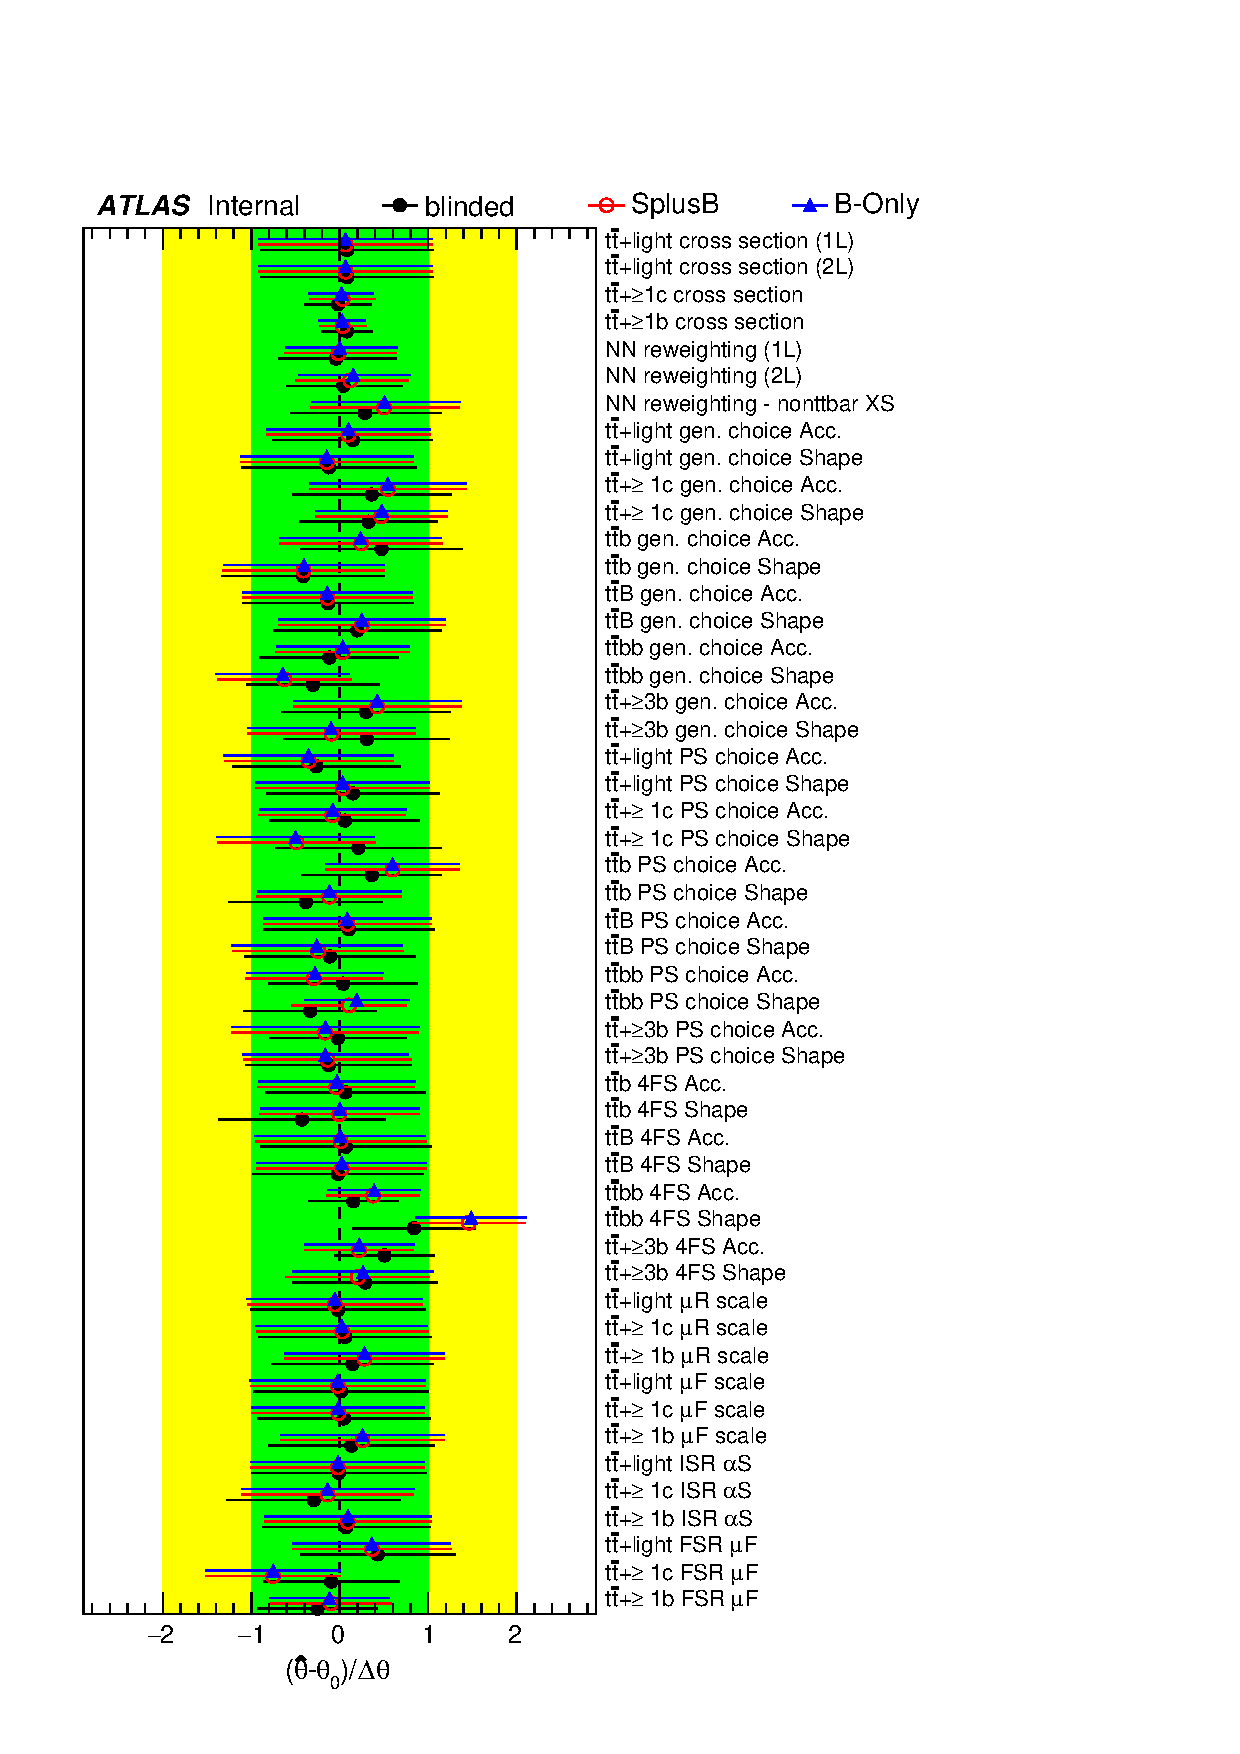
\includegraphics[width=\linewidth]{figures/fits/comparisons/fitTypes/1000/all/comparison_data/NuisPar_comp_ttbar.pdf}
    \subcaption{mH=1000\gev}
  \end{subfigure}
  \caption{\label{fig:comparison_NP_ttbar}Fitted pulls and constraints for the nuisance parameters corresponding to the \ttbar systematic uncertainties for combined Data fits for three mass points. Comparison is done for three fits: blinded background-only data fit, unblinded background-only data fit, and unblinded signal+background data fit.}
\end{figure}

\begin{figure}[htbp!]
  \centering
  \begin{subfigure}[t]{0.32\textwidth}
    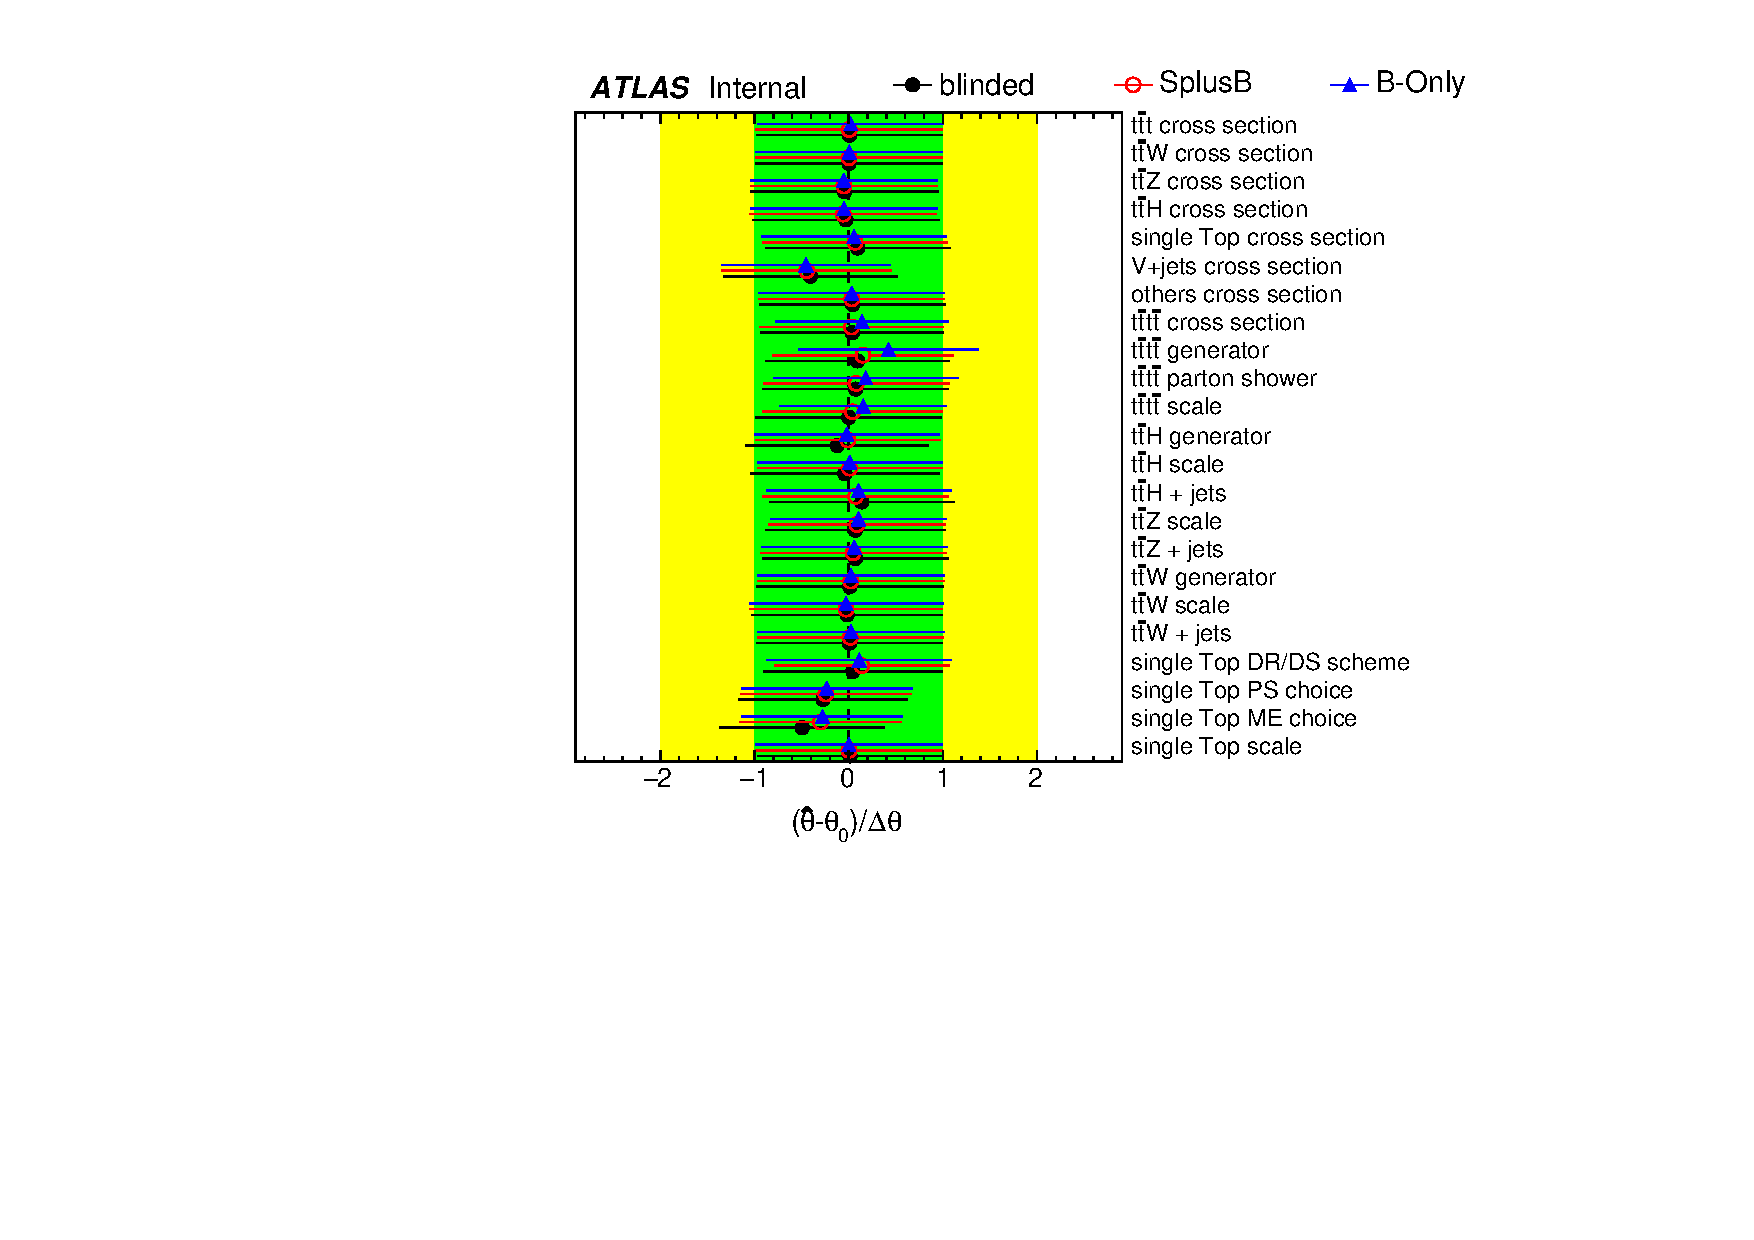
\includegraphics[width=\linewidth]{figures/fits/comparisons/fitTypes/400/all/comparison_data/NuisPar_comp_Other.pdf}
    \subcaption{mH=400\gev}
  \end{subfigure}
  \begin{subfigure}[t]{0.32\textwidth}
    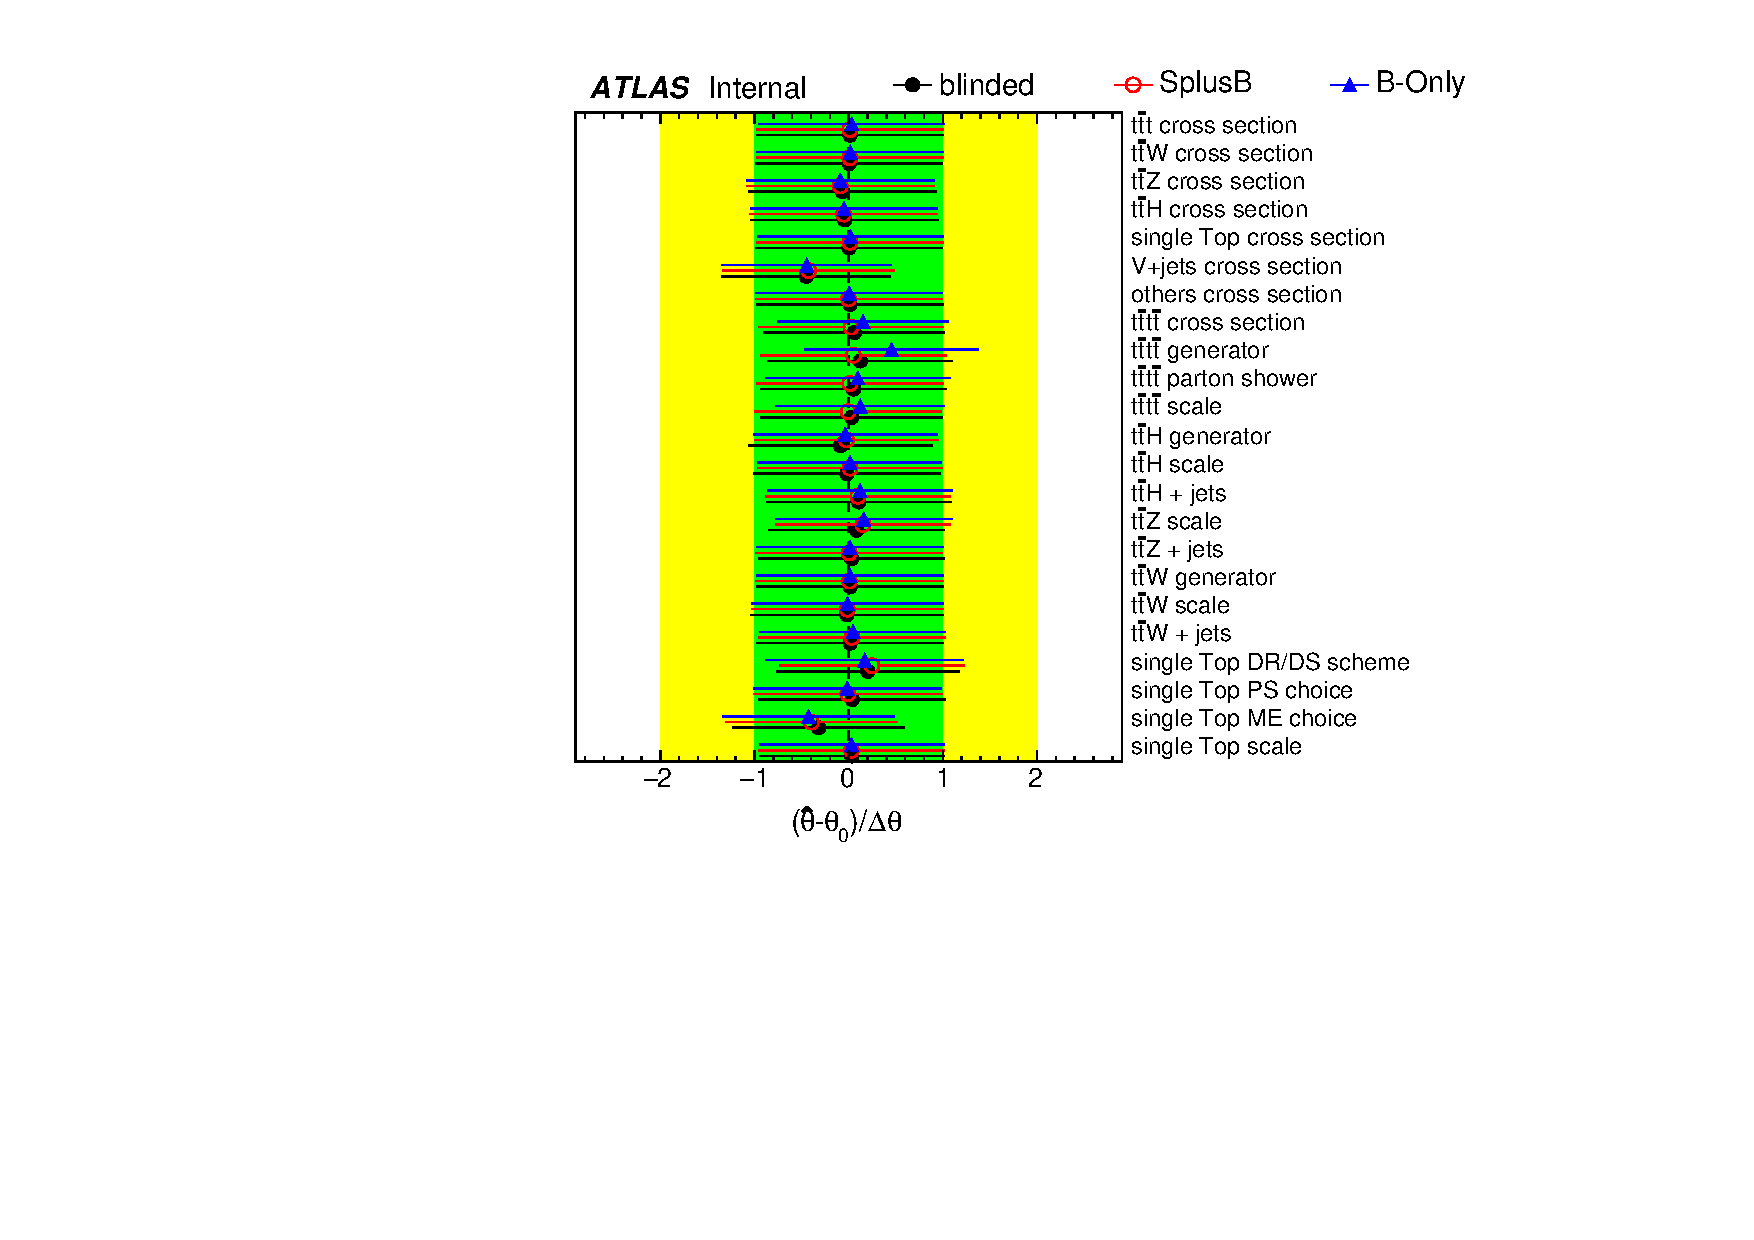
\includegraphics[width=\linewidth]{figures/fits/comparisons/fitTypes/700/all/comparison_data/NuisPar_comp_Other.pdf}
    \subcaption{mH=700\gev}
  \end{subfigure}
  \begin{subfigure}[t]{0.32\textwidth}
    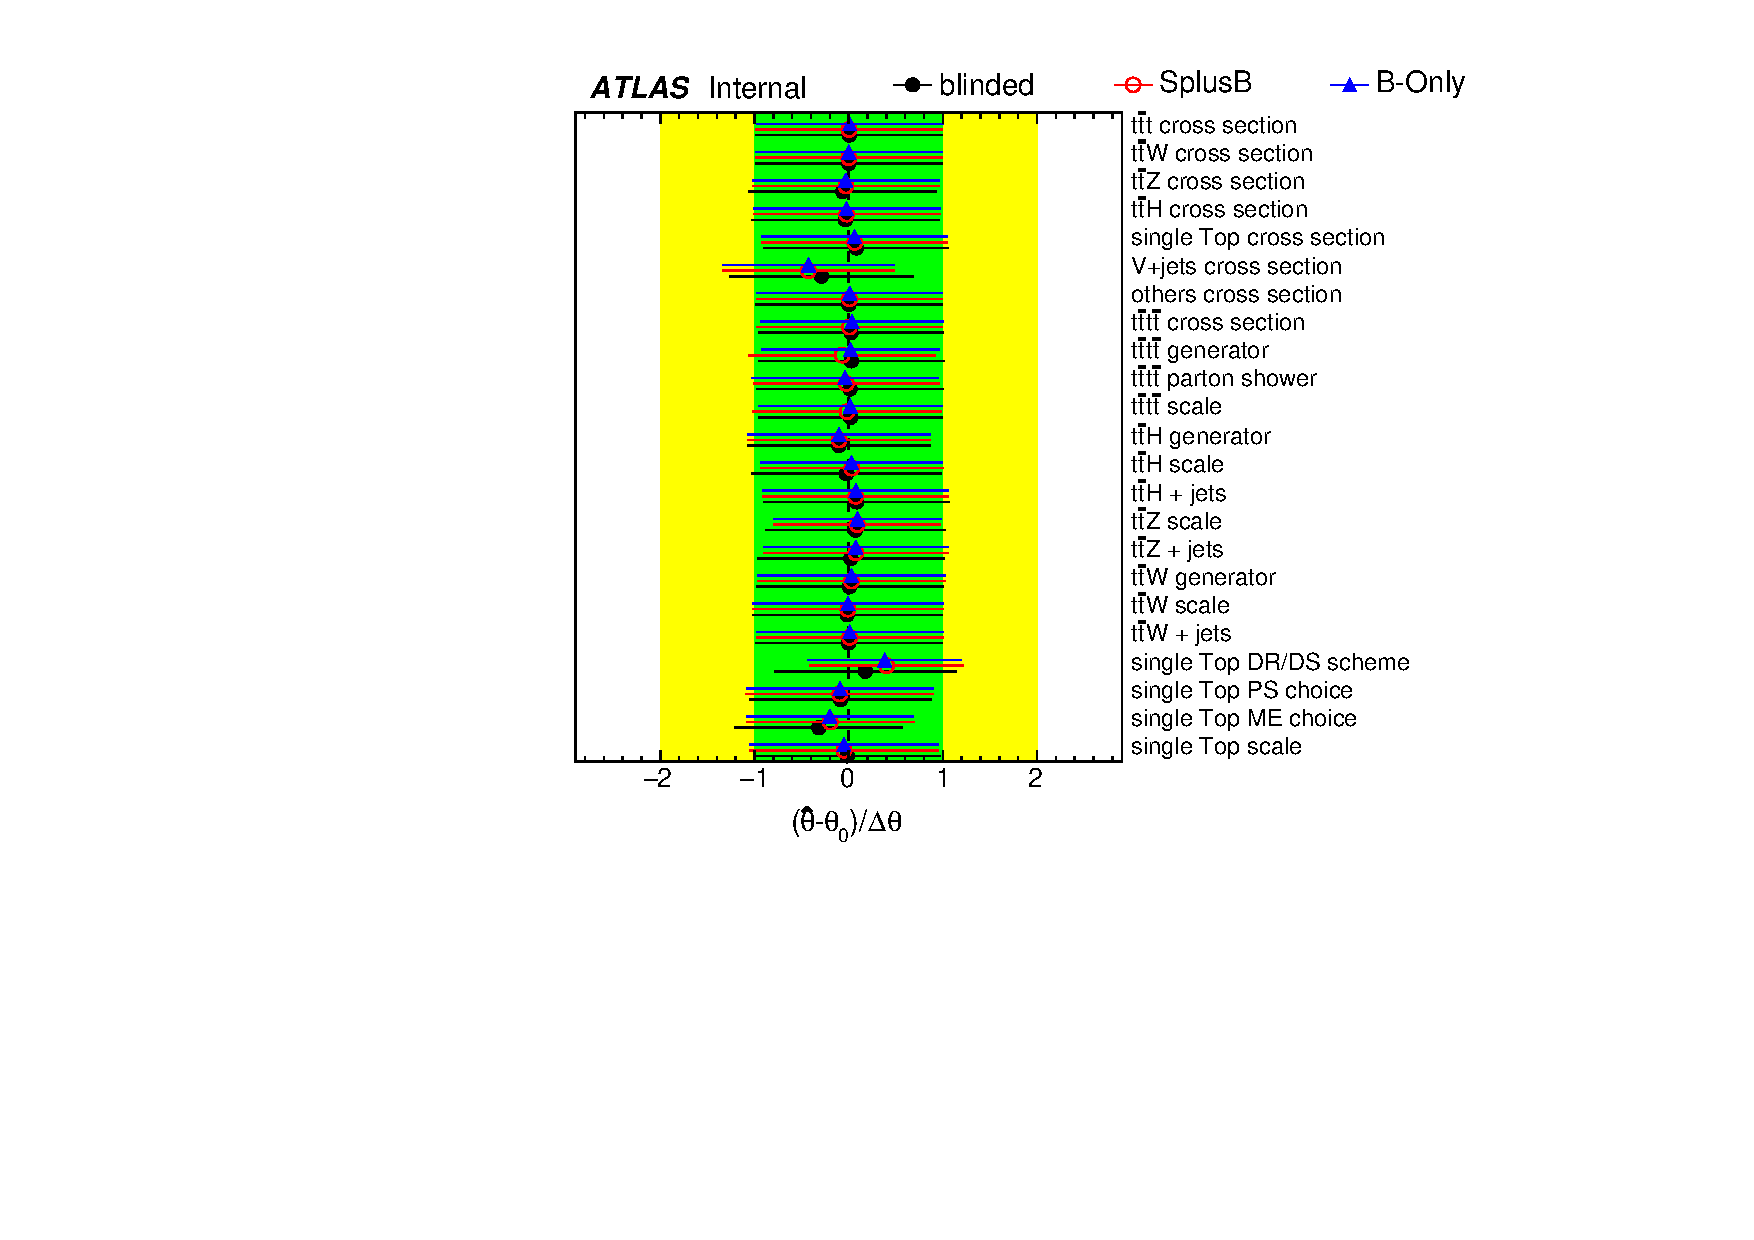
\includegraphics[width=\linewidth]{figures/fits/comparisons/fitTypes/1000/all/comparison_data/NuisPar_comp_Other.pdf}
    \subcaption{mH=1000\gev}
  \end{subfigure}
  \caption{\label{fig:comparison_NP_other}Fitted pulls and constraints for the nuisance parameters corresponding to the non-\ttbar background systematic uncertainties for combined Data fits for three mass points. Comparison is done for three fits: blinded background-only data fit, unblinded background-only data fit, and unblinded signal+background data fit.}
\end{figure}


\subsection{Goodness of fit vs mass}
The figure \ref{fig:goodnessOfFit_mass} shows the goodness of fit evaluation for unblinded fits (signal+background and Background-only) as a function of mass of hypothetical heavy higgs boson in all regions $(1L+2LOS)$ regions.
\begin{figure}[htbp!]
        \centering
        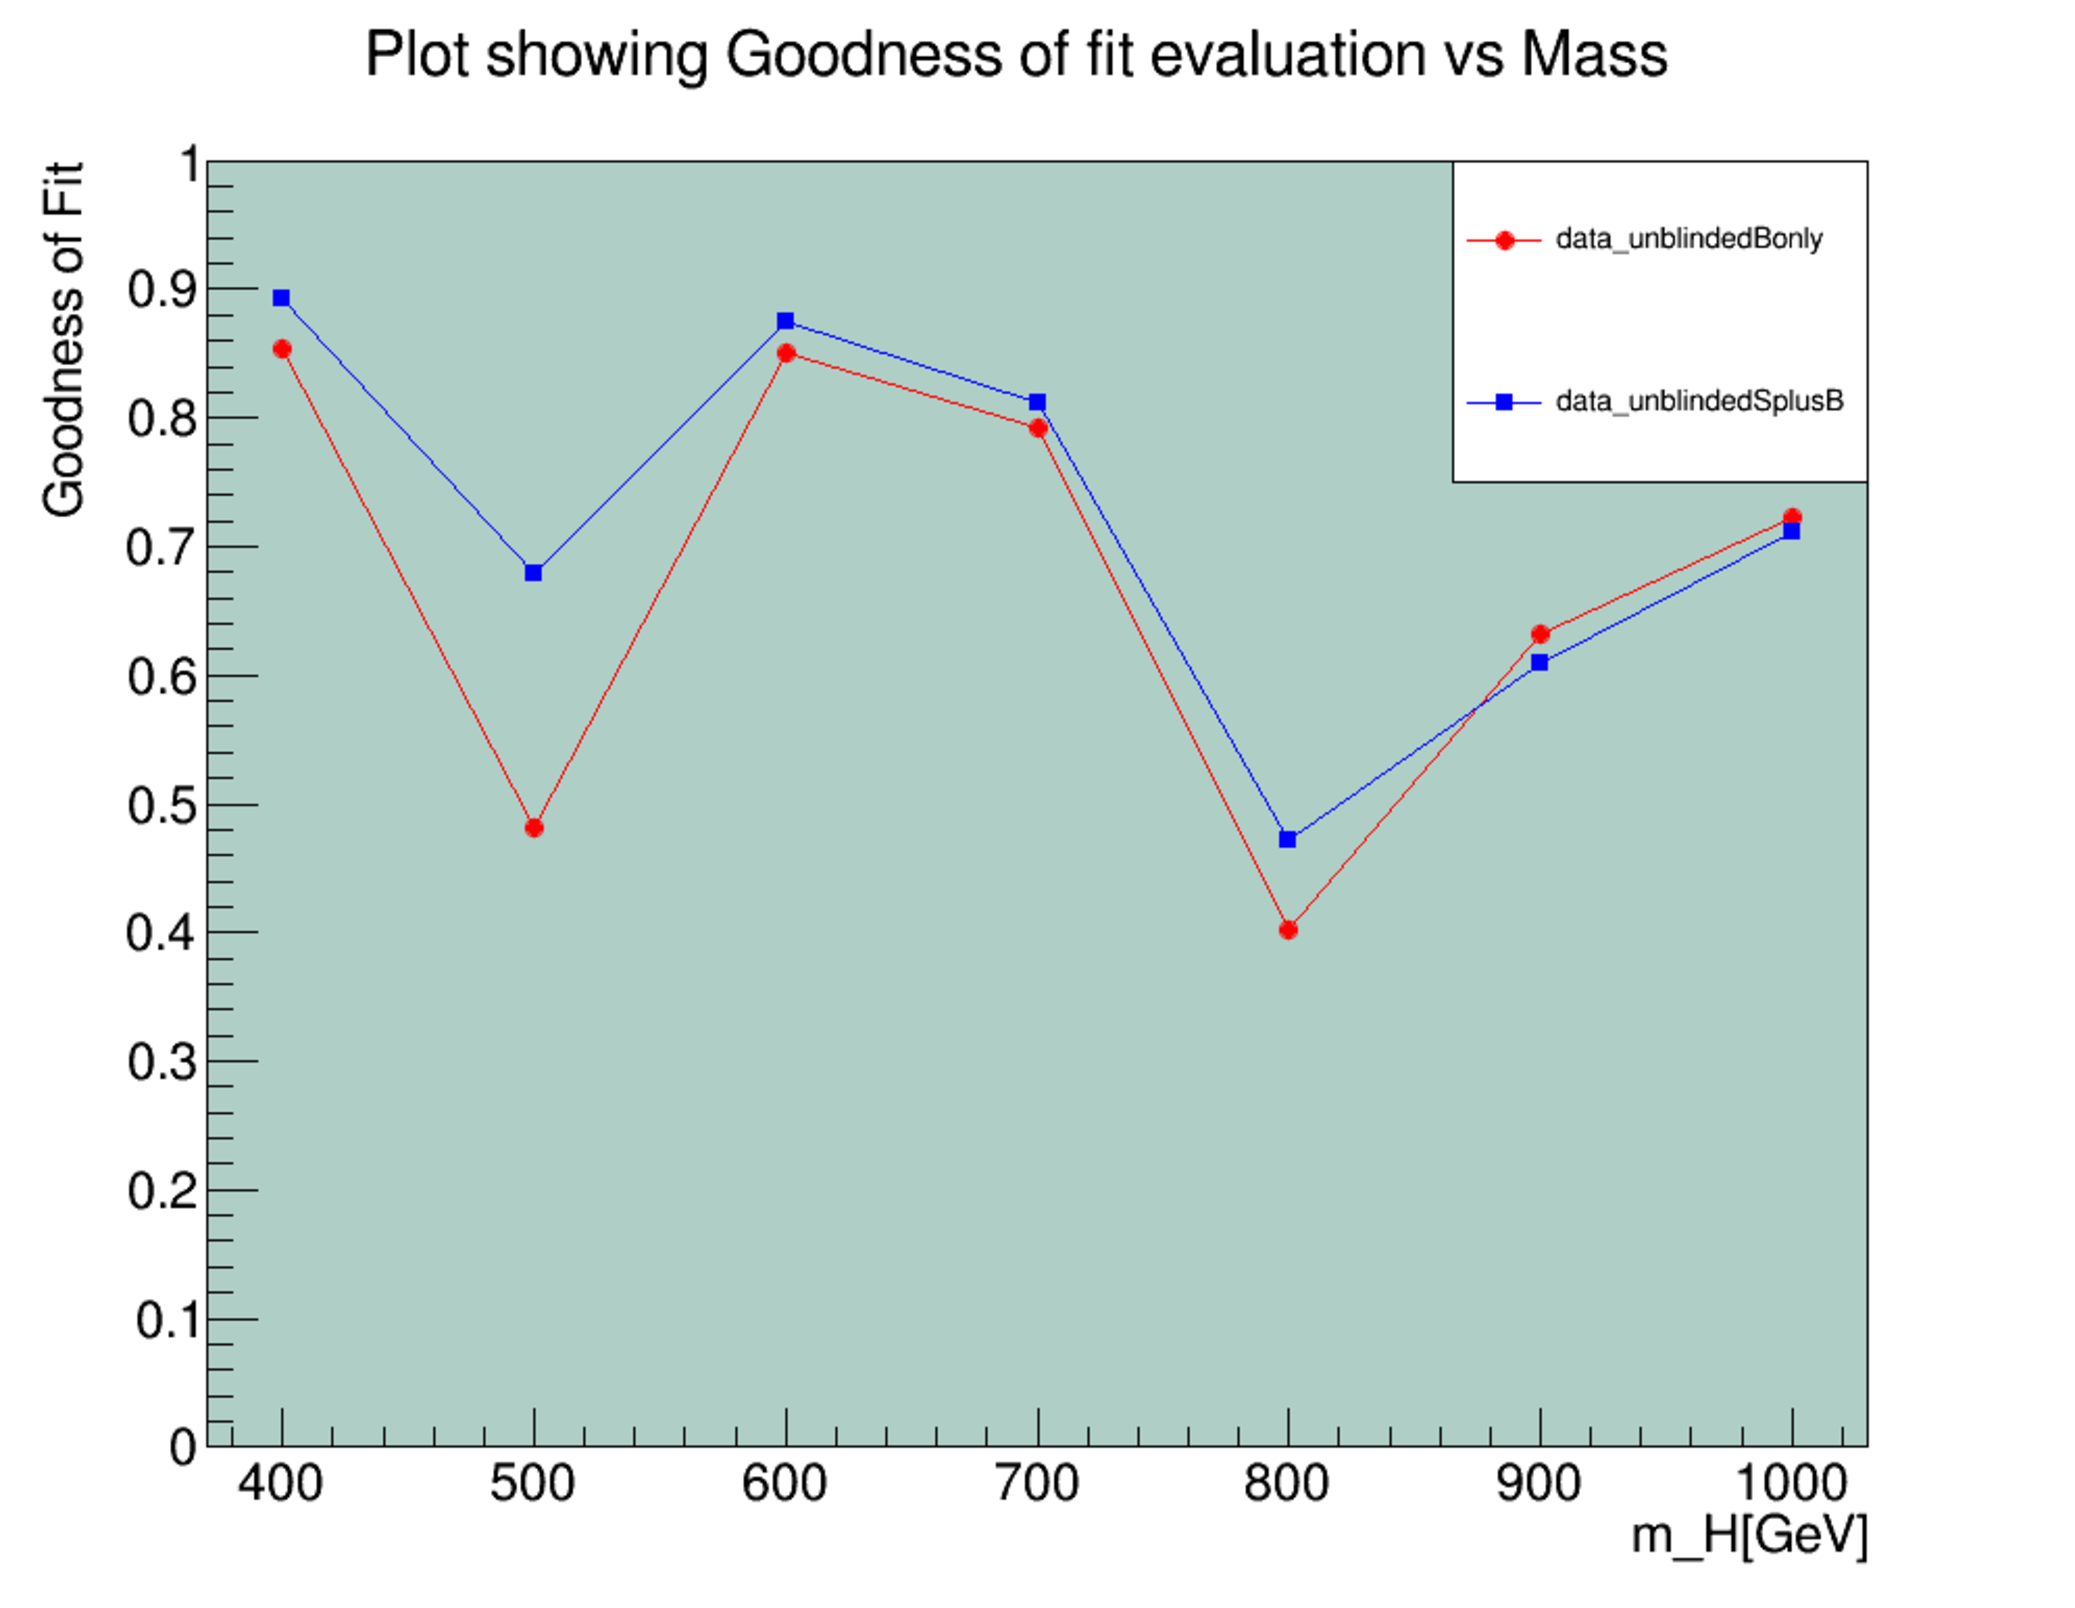
\includegraphics[width=\linewidth]{figures/fits/comparisons/goodnessVsMass.pdf}
        \caption{\label{fig:goodnessOfFit_mass} Comparison among unblinded fits (signal+background and Background-only)in all regions as a function of mass of hypothetical heavy higgs boson $m_{H}$(GeV) }
\end{figure} 
